\documentclass[11pt]{article}
\usepackage{geometry}                % See geometry.pdf to learn the layout options. There are lots.
\geometry{letterpaper}                   % ... or a4paper or a5paper or ... 
%\geometry{landscape}                % Activate for for rotated page geometry
\usepackage[parfill]{parskip}    % Activate to begin paragraphs with an empty line rather than an indent
\usepackage{graphicx}
\usepackage{amssymb}
\usepackage{epstopdf}
\usepackage[usenames,dvipsnames]{color}
\usepackage{fancyvrb}
\usepackage{listings}
\usepackage{booktabs,footmisc}
\usepackage{hyperref}
\usepackage[all]{hypcap}

\usepackage{topcapt}
\usepackage{hyperref}


 
% include the lines below to use a nicer fixed-width font than the default one
 
\lstset{fancyvrb=true}
\lstset{
	basicstyle=\small\tt,
	identifierstyle=,
	commentstyle=\color{Bittersweet},
	stringstyle=\color{red},
	showstringspaces=false,
	tabsize=2,
	numbers=none,
	captionpos=b,
	xleftmargin=2em,
	frame=single,
	breaklines=true
%	numberstyle=\tiny
	%stepnumber=4
	}
\DeclareGraphicsRule{.tif}{png}{.png}{`convert #1 `dirname #1`/`basename #1 .tif`.png}


\title{Repast Simphony Frequently Asked Questions}
\author{Repast Development Team}


\begin{document} 
\maketitle

\section{General Questions}
\begin{itemize}
\item \nameref{gq:domain_of_interest}
\item \nameref{gq:rj_vs_rs}
\item \nameref{gq:training}
\item \nameref{gq:nl_import}
\end{itemize}

\section{Programming with Repast Simphony}
\begin{itemize}
\item \nameref{prs:examples}
\item \nameref{prs:schedule_global}
\item \nameref{prs:custom_display}
\item \nameref{prs:ae_groovy}
\item \nameref{prs:convert}
\item \nameref{prs:convert_j}
\item \nameref{prs:rs_in_java}
\item \nameref{prs:schedule_java}
\item \nameref{prs:regression}
\item \nameref{prs:neural_network}
\item \nameref{prs:genetic}
\item \nameref{prs:system_dynamics}
\item \nameref{prs:mat_lab}
\item \nameref{prs:model_score}
\item \nameref{prs:3d_models}
\end{itemize}


\section{Problems}
\begin{itemize}
\item \nameref{p:combo}
\item \nameref{p:classpath}
\item \nameref{p:run}
\item \nameref{p:log4j}
\item \nameref{p:mem}
\item \nameref{p:amts}
\item \nameref{p:r}
\item \nameref{p:copy_paste}
\item \nameref{p:slow}
\item \nameref{p:nvidia}
\item \nameref{p:missing_project}
\end{itemize}


\setcounter{section}{0}
\section{General Questions}
\subsection{How can I create an agent-based model in my domain of interest?}
\label{gq:domain_of_interest}
Agent-based models are not necessarily complicated or hard to make, but there is no single modeling approach that works for all domains. To get a better understanding of agent-based modeling and simulation (ABMS) and ABMS toolkits, take a look at the proceedings from the Agent 200X conference \url{http://www.dis.anl.gov/agent20XY/}.

Additionally, a new book is available on how to do agent-based modeling and simulation. The book is titled Managing Business \begin{enumerate}
\item how to think about agent-based modeling, that is, about agents and their interactions;
\item how to explain the features and advantages of agent-based modeling to other people;
\item and how to actually implement agent-based simulations.
\end{enumerate}
The new book is intended to be a complete agent-based modeling resource, accessible to readers who haven't had any previous experience in building agent-based simulations, or any other kinds of models, for that matter.
The book's details are as follows:\\\\
Title: {\bf Managing Business Complexity: Discovering Strategic Solutions with Agent-Based Modeling and Simulation}\\
Authors: Michael J. North and Charles M. Macal Publisher: Oxford University Press\\
Publication Date: March 2007\\ 
ISBN: 0-19-517211-6\\

The book's table of contents is as follows:
\begin{enumerate}
\item The Challenge 
\item The ABMS Paradigm
\item Agents Up Close 
\item The Roots of ABMS 
\item The Role of ABMS 
\item Discovering Agents and Agent Behaviors 
\item Office ABMS 
\item How to Do Desktop ABMS 
\item How to Do Participatory ABMS
\item How to Do Large-Scale ABMS 
\item ABMS Verification and Validation 
\item A Visual Approach to Data Collection and Cleaning 
\item Understanding and Presenting ABMS Results 
\item ABMS Project Management 
\item Rising to the Challenge
\end{enumerate}

Further information on the book can be found at the following address:
\url{http://tinyurl.com/2sgtlc}

\subsection{What is the difference between Repast J and Repast Simphony?}
\label{gq:rj_vs_rs}
Repast Simphony is a free and open source agent-based modeling toolkit that offers users a rich variety of features including the following:
\begin{enumerate}
\item An optional point-and-click model development environment that generates Java classes and seamlessly integrates with hand written Java and Groovy components.
\item A pure Java point-and-click model execution environment that includes built-in results logging and graphing tools as well as automated connections to a variety of optional external tools including R, VisAD, Weka, popular spreadsheets, MATLAB, and iReport.
\item An extremely flexible hierarchically nested definition of space including the ability to do point-and-click and modeling and visualization of 2D environments, 3D environments, networks including full integration with the JUNG network modeling library, and geographical spaces including full Geographical Information Systems (GIS) support.
\item A range of data storage "freeze dryers" for model check pointing and restoration including text file and database storage.
\item A fully concurrent multithreaded discrete event scheduler. 
\item Libraries for genetic algorithms, neural networks, regression, random number generation, and
specialized mathematics.
\item Automated Monte Carlo simulation framework which supports multiple modes of model results
optimization. 
\item Built-in tools for integrating external models. 
\item Fully object-orientation.
\item Availability on virtually all modern computing platforms including Windows, Mac OS, and Linux.
\end{enumerate}

More information on Repast Simphony can be found on the main web site:  \url{https://repast.github.io}.
You might look at the following papers in the Agent 2006 proceedings at \url{http://www.dis.anl.gov/agent20XY/proceedings/Agent2006.pdf}

Howe, T.R., N.T. Collier, M.J. North, M.T. Parker, and J.R. Vos, "Containing Agents: Contexts, Projections, and Agents," Proceedings of the Agent 2006 Conference on Social Agents: Results and Prospects, Argonne National Laboratory, Argonne, IL USA (September 2006).

North, M.J., P. Sydelko, J.R. Vos, T.R. Howe, and N.T. Collier, "Legacy Model Integration with Repast Simphony," Proceedings of the Agent 2006 Conference on Social Agents: Results and Prospects, Argonne National Laboratory, Argonne, IL USA (September 2006).

Parker, M.T., T.R. Howe, M.J. North, N.T. Collier, and J.R. Vos, "Agent-Based Meta-Models," Proceedings of the Agent 2006 Conference on Social Agents: Results and Prospects, Argonne National Laboratory, Argonne, IL USA (September 2006).

Tatara, E., M.J. North, T.R. Howe, N.T. Collier, and J.R. Vos, "An Introduction to Repast Modeling by Using a Simple Predator-Prey Example," Proceedings of the Agent 2006 Conference on Social Agents: Results and Prospects, Argonne National Laboratory, Argonne, IL USA (September 2006).

\subsection{Are training courses available for Repast Simphony?}
\label{gq:training}
We typically offer three days of training in Chicago, IL USA at the Agent 20XY (\url{http://www.dis.anl.gov/agent20XY/}) conference. We also run an intensive business-oriented ABMS course in Chicago, IL USA which includes two and a half days of Repast training (\url{http://www.dis.anl.gov/conferences/abms/info.html}). Other short courses are scheduled periodically in other areas.

\subsection{How do I import a NetLogo model?}
\label{gq:nl_import}
Repast Simphony offers a \href{http://ccl.northwestern.edu/netlogo/}{NetLogo} model import wizard which can be activated as follows:
\begin{itemize}
\item Select File $\rightarrow$ Import... from the Eclipse main menu
\item Open the ReLogo category
\item Select the NetLogo Model option
\item Click Next
\item Browse to or input the *.nlogo file name
\item Select only shapes that are licensed to you (e.g., those you've created) (Please note that ReLogo offers a set of default shapes for your use)
\item Click Finish
\end{itemize}

Your model now has been converted to ReLogo. You may find that there are a small number of updates to be made to the code to run your new model. These updates are necessitated by the object oriented nature of ReLogo and the Repast Simphony modeling environment. We note that future updates to the NetLogo system, which are beyond our control, may ameliorate or exacerbate this situation.

Please see the ReLogo Getting Started Guide for information on how to operate and extend your model.
\section{Programming with Repast Simphony}

\subsection{Where can I find example models for Repast Simphony}
\label{prs:examples}
Repast Simphony offers a number of example models that you can import and run as follows:
\begin{itemize}
\item Select File $\rightarrow$ Import Repast Examples from the Eclipse main menu
\item Check the boxes for the example projects you would like to import
\item Click Finish
\end{itemize}

The example project has now been copied to your workspace and can be modified as needed (without affecting the original example model).

\subsection{How do I schedule a ``global'' behavior, a behavior above the individual agent level?}
\label{prs:schedule_global}

There's at least two ways to do this. Both assume that you create your model in your own ContextBuilder.

The first way requires that you have your ContextBuilder extend DefaultContext. Once you've done this you can add @ScheduledMethods to this ContextBuilder to perform some global action.

\noindent\begin{minipage}[h]{\textwidth}
\vspace{.2in}
\lstset{language=java}
\begin{lstlisting}
public class MyContextBuilder extends DefaultContext 
	implements ContextBuilder {

	/**
	 * Builds and returns a context. Building a context consists of filling 
	 * it with agents, adding projects and so forth. The returned context
	 * does not necessarily have to be the passed in context.
	 *
	 * @param context
	 * @return the built context.
	 */
	public Context build(Context<T> context) {
		...
	}
	
	@ScheduledMethod(start = 1)
	 public void step() {
	   	// my "global" behavior
	 }
}
\end{lstlisting}
\vspace{.2in}
\end{minipage}

The second way uses the RunEnvironment object to get a reference to the current Schedule with which can add your behavior. For example,

\noindent\begin{minipage}[h]{\textwidth}
\vspace{.2in}
\lstset{language=java}
\begin{lstlisting}
public class MyContextBuilder implements ContextBuilder {

	public Context build(Context<T> context) {
		...
		ISchedule schedule = RunEnviroment.getCurrentSchedule();
		ScheduleParameters params = ScheduleParameters.createOneTime(1);
		schedule.schedule(params, this, "step");
	}

 	public void step() {
   		// my global behavior
 	}
}
\end{lstlisting}
\vspace{.2in}
\end{minipage}

Note that while the above schedules the execution of MyContextBuilder.step, any of the options provided by ISchedule are available.

\subsection{How do I create a custom display?}
\label{prs:custom_display}

All simphony displays implement IDisplay. \href{https://repast.github.io/docs/CustomDisplay.java}{CustomDisplay.java} is an example that displays a panel with a simple label in it. Note that most of the methods are empty or return null. The important methods are render, update and getPanel. When update is called the display should update its internal state to reflect the latest state of whatever its displaying. When render is called, the display should draw those updates. getPanel is called during initialization to put a panel into a display tab.

The next step then is telling simphony to load this display during initialization. You do that with a ModelInitializer. The model initializer is run once just after your scenario is loaded. It can be used to add additional items to the scenario tree that's displayed on the left hand side of simphony. Its not immediately obvious but this is actually a tree of actions that simphony executes when it initializes a model prior to a run. A model initializer then can add a custom action that initializes a custom display.  \href{https://repast.github.io/docs/TrapInitializer.java}{TrapInitializer.java} does just that. The second added controller action is what sets up the custom display. Lastly, you need tell Simphony to run your ModelInitializer and you do that in the scenario.xml file located in your scenario directory (e.g. mousetrap.rs) by adding a model.initializer entry. For example,

$\langle$model.initializer class="repast.simphony.demo.mousetrap.TrapInitializer"$\rangle$

\subsection{Do I have to use the agent editor and Groovy for my agents?}
\label{prs:ae_groovy}

No. Repast Simphony accepts both user defined POJOs (Plain Old Java Objects) as well as POGOs (Plain Old Groovy Objects) as agents (or for defining other model components), making the use of Groovy completely optional. The graphical agent behavior editor generates Groovy agent classes. For those interested in learning more about Groovy, a dynamically typed programming language very well integrated with Java, there is the Groovy home page \url{http://groovy.codehaus.org/} and the very informative book "Groovy in Action" by Dierk Koenig.

\subsection{How can I convert my Repast Simphony 1.0, 1.1 or 1.2 model to run in Repast Simphony 2.0?}
\label{prs:convert}

To upgrade scenarios simply do the following:

\begin{itemize}
\item Right click on the scenario folder (usually "yourmodelname.rs").
\item Choose "Convert Scenario" from the popup menu.
\end{itemize}

This will create a user\_path.xml and a context.xml from your old Score file. It will also make backup copy of the scenario.xml file and then remove any displays from the scenario file. Removing the displays is necessary because old Piccolo 2D displays will no longer load in version 2.0.

\subsection{How can I convert my Repast J model to run in Repast Simphony?}
\label{prs:convert_j}

A quick summary of the process of converting to Repast J to Repast S:
\begin{itemize}
\item Create a new Repast Simphony project or add the Repast nature to your existing project(see tutorial).
\item Strip out all of the Repast J-specific visualization code from your agents (ie extends DefaultDrawableNode).
\item Pick out the relative information such as scheduling and model parameters from the Repast J main class (ie SimpleModelImpl) and put this in the Repast S ContextBuilder or agent class constructors (where ever you see fit).
\item Create a scenario/score model.
\item Create displays, loggers, etc via the Repast S runtime interface.
\end{itemize}

Several of the demos (sugarscape and regression) included with Repast S are direct ports from the Repast J models, so comparing these will provide some additional help on porting models.

\subsection{How can I run Repast Simphony from another Java application?}
\label{prs:rs_in_java}

Repast may be launched programmatically by directly calling the repast.simphony.runtime.RepastMain class. RepastMain takes two arguments, the first is the location of the model scenario directory and the second is an optional location of the repast runtime location.

Note that you need to have repast.simphony.runtime/bin and the jars in repast.simphony.runtime/lib on your classpath since the runtime needs these to start.

Also, you can put the repast runtime folders anywhere you like if you are calling the RepastMain from your own code. As long as you have repast.simphony.runtime/bin to your classpath, RepastMain will be able to find the runtime and start properly.

Here's a simple class that will do this:

\noindent\begin{minipage}[h]{\textwidth}
\vspace{.2in}
\lstset{language=java}
\begin{lstlisting}
public class UserMain {

public UserMain(){};

  public void start(){

    String[] args = new String[]{"C:/myModel/scenario.rs"};

    repast.simphony.runtime.RepastMain.main(args);
  }

  public static void main(String[] args) {

    UserMain um = new UserMain();
    um.start();
  }
}
\end{lstlisting}
\vspace{.2in}
\end{minipage}


\subsection{How can I control the Repast Simphony schedule from another Java application?}
\label{prs:schedule_java}
To run a simulation purely programmatically with fine control, you need to create a class that extends repast.simphony.engine.environment.AbstractRunner and modify to suit your needs. The runner class can then be used to initialize, step, run, pause, stop and reset the model. This approach uses components from the GUI which is totally user driven and the Batch run which is completely self-contained with no user-interaction.

\href{https://repast.github.io/docs/TestRunner_2.java}{TestRunner\_2.java} and main class \href{https://repast.github.io/docs/TestMain_2.java}{TestMain\_2.java}. In this case you won't use either the RepastMain (GUI) or the BatchMain (batch mode), but use the runner class directly. Note that you will need to include the classes from repast.simphony.runtime and repast.simphony.Batch in your classpath to run.

\subsection{How can I implement regression in Repast Simphony?}
\label{prs:regression}
Repast Simphony (Repast S) uses the OpenForecast (\url{http://openforecast.sourceforge.net/}) library to implement regression. OpenForecast can be used directly within agents or the Repast S regression wrapper can be used. Directly using OpenForecast provides maximum flexibility but requires more complex programming. The Repast S regression wrapper simplifies the use of OpenForecast while preserving most options. It is recommended that Repast S users start with the Repast S wrapper and, only if needed, eventually move to directly use of OpenForecast. The Repast S regression wrapper is consistent with direct use of OpenForecast so this should relatively straightforward. Obviously, as with all statistical tools, it is important to make sure that regression, in general, and the chosen regression fit, in particular, are appropriate for your application. The method "getForecastType()" can be used to find a text description of the selected equation for both types of regression. It is recommended that this be checked for appropriateness.

Documentation on how to use OpenForecast directly can be found on their web site, \url{http://openforecast.sourceforge.net/}

To use the Repast S regression wrapper in the visual editor simply follow these steps:
\begin{enumerate}
\item Add a property of type "Multilinear Regression Model" or "Best Fit Regression Model" to an agent "Multilinear Regression Model" always fits input data sets using a linear equation for one input variable or multilinear equation for multiple input variables. "Best Fit Regression Model" causes OpenForecast to consider a range of different equation families and then find the best fitting member of the best fitting equation family. This includes linear and multilinear equations as well as other families as defined in the OpenForecast documentation.
\item Using the Wizard dialog, chose "Advanced Adaptation," "Use a Regression Model," "Store Data for a Regression Model," and then fill in the form to store data for fitting.
\item Using the Wizard dialog, chose "Advanced Adaptation," "Use a Regression Model," "Forecast from a Regression Model," and then fill in the form to get a forecast. Please note that it generally is necessary to return default forecasts for several steps before enough example data is available for a good quality forecast.
\end{enumerate}

To use the Repast S regression wrapper in the Java or Groovy simply follow these steps:
\begin{enumerate}
\item Add an agent class field of type RepastRegressionModel and create an instance (i.e., new RepastRegressionModel(false)). Set the constructor parameter to "false" for "Multilinear Regression Model" or "true" for "Best Fit Regression Model." "Multilinear Regression Model" always fits input data sets using a linear equation for one input variable or multilinear equation for multiple input variables. "Best Fit Regression Model" causes OpenForecast to consider a range of different equation families and then find the best fitting member of the best fitting equation family. This includes linear and multilinear equations as well as other families as defined in the OpenForecast documentation. Obviously, as with all statistical tools, it is important to make sure that the chosen functions, both multilinear and best fit, are appropriate for your application. The method "getForecastType()" can be used to find a text description of the selected equation for both types of regression. It is recommended that this be checked for appropriateness.
\item Use the new field's "add(...) method to store data for fitting (i.e., model.add(y, x1, x2, x3)).
\item Use the new field's "forecast(...)" method to get a forecast (i.e., double x = model.forecast(y1, y2, y3)). Please note that it generally is necessary to return default forecasts for several steps before enough example data is available for a good quality forecast.
\end{enumerate}

\subsection{How can I implement neural networks in Repast Simphony?}
\label{prs:neural_network}

Repast Simphony (Repast S) uses the Java Object Oriented Neural Engine (Joone) (\url{http://www.jooneworld.com/}) library to implement neural networks. Joone can be used directly within agents or the Repast S neural network wrapper can be used. Directly using Joone provides maximum flexibility but requires more complex programming. The Repast S wrapper simplifies the use of Joone while preserving most options. It is recommended that Repast S users start with the Repast S wrapper and, only if needed, eventually move to directly use of Joone. The Repast S wrapper is consistent with direct use of Joone so this should relatively straightforward. Obviously, as with all machine learning tools, it is important to make sure that neural networks, in general, and the chosen network design, in particular, are appropriate for your application.

Documentation on how to use Joone directly can be found on their web site, \url{http://www.jooneworld.com/}.

To use the Repast S neural network wrapper in the visual editor simply follow these steps:
\begin{enumerate}
\item Add a property of type "Linear Neural Network," "Logistic Neural Network," or "Softmax Neural Network" to an agent to produce the corresponding type of neural network. Replace the integer (i.e., int) array elements with a description of the layers for your application. The first number in the array is the count of input neurons, the last number is the count of output neurons, and the intermediate numbers are the interstitial layers. You can have as many interstitial layers as you would like (i.e., zero or more).
\item Using the Wizard dialog, chose "Advanced Adaptation," "Use a Neural Network," "Train a Neural Network Model," and then fill in the form to store data for fitting. The input data array is indexed by the number of training examples and the number of input neurons. The output data array is indexed by the number of training examples and the number of output neurons.
\item Using the Wizard dialog, chose "Advanced Adaptation," "Use a Neural Network," "Forecast from a Neural Network," and then fill in the form to get a forecast. The input data array is indexed by the number of input neurons. The output data array is indexed by the number of output neurons.
\end{enumerate}

To use the Repast S regression wrapper in the Java or Groovy simply follow these steps:
\begin{enumerate}
\item Add an agent class field of type NeuralNet and create an linear, logistic, or softmax instance as follows:

JooneTools.create\_standard(new int[]{inputNeurons intermediateLayer1 intermediateLayer2 intermediateLayerN outputNeurons}, JooneTools.LINEAR)).

JooneTools.create\_standard(new int[]{inputNeurons intermediateLayer1 intermediateLayer2 intermediateLayerN outputNeurons}, JooneTools.LOGISTIC)).

JooneTools.create\_standard(new int[]{inputNeurons intermediateLayer1 intermediateLayer2 intermediateLayerN outputNeurons}, JooneTools. SOFTMAX)).

\item Use the following method to store data for fitting where "model" is the new field name:

JooneTools.train(model, inputDataArray, targetOutputDataArray, epochs, convergenceLimit, 0, null);

The input data array is indexed by the number of training examples and the number of input neurons. The output data array is indexed by the number of training examples and the number of output neurons. The model will be trained until "epochs" cycles are completed or the "convergenceLimit" of root mean square error is achieved, whichever comes first.
\item Use the following method to get a forecast where "model" is the new field name:

double outputData[] = JooneTools.interrogate(model, inputData)
\end{enumerate}

The input data array is indexed by the number of input neurons. The output data array is indexed by the number of output neurons.

\subsection{How can I implement genetic algorithms in Repast Simphony?}
\label{prs:genetic}

Repast Simphony (Repast S) uses the Java Genetic Algorithms Package (JGAP) (\url{http://jgap.sourceforge.net/}) to implement genetic algorithms. JGAP can be used directly within agents or the Repast S genetic algorithms (GA) wrapper can be used. Directly using JGAP provides maximum flexibility but requires more complex programming. The Repast S GA wrapper simplifies the use of JGAP while preserving most options. It is recommended that Repast S users start with the Repast S wrapper and, only if needed, eventually move to directly use of JGAP. The Repast S regression wrapper is consistent with direct use of JGAP so this should relatively straightforward. Obviously, as with all machine learning tools, it is important to make sure that genetic algorithms, in general, and the chosen formulation, in particular, are appropriate for your application.

Documentation on how to use JGAP directly can be found on their web site, \url{http://jgap.sourceforge.net/}. In particular, please see the following page:

\url{http://jgap.sourceforge.net/doc/tutorial.html}

To use the Repast S GA wrapper in the visual editor simply follow these steps:

\begin{enumerate}
\item Add a property of type "Genetic Algorithm" to an agent. "evaluate" is the name of the fitness function that needs to be created as described in step two. "populationSize" is the count of the members in the GA population. The "Gene" array gives the set of genes, either "IntegerGene" or "DoubleGene," to be used. The parameters to the constructors (e.g., "min1" and "max1") are the optional lower and upper bounds for that gene. The template is as follows:

new RepastGA(this, "evaluate", populationSize, new Gene[]{ new IntegerGene(min1, max1) new DoubleGene(min2, max2)})

\item Add a behavior that takes a double precision array (i.e., "double[]"), returns an positive integer result, and that uses the fitness function name given above (e.g., "evaluate"). The double array is the current population member to be evaluated. The genes are in the same order as the template given in step one. Higher fitness result values mean greater fitness levels. The exact range does not matter as long as the numbers are positive.

\item Using the Wizard dialog, chose "Advanced Adaptation," "Use a Genetic Algorithm," "Get the Best Solution from a Genetic Algorithm," and then fill in the form to get a solution. The returned double array is the current best solution. The genes are in the same order as the template given in step one.

\item f the population needs to be reset, perhaps due to a plateau, using the Wizard dialog, chose "Advanced Adaptation," "Use a Genetic Algorithm," "Reset the Population of a Genetic Algorithm," and then fill in the form.
\end{enumerate}

To use the Repast S GA wrapper in the Java or Groovy simply follow these steps:
\begin{enumerate}
\item Add an agent class field of type RepastGA and create an instance following this template:

new RepastGA(this, "evaluate", populationSize, new Gene[]{ new IntegerGene(min1, max1) new DoubleGene(min2, max2)})

"evaluate" is the name of the fitness function that needs to be created as described in step two. "populationSize" is the count of the members in the GA population. The "Gene" array gives the set of genes, either "IntegerGene" or "DoubleGene," to be used. The parameters to the constructors (e.g., "min1" and "max1") are the optional lower and upper bounds for that gene.
\item Add a class method behavior that takes a double precision array (i.e., "double[]"), returns an positive integer result, and that uses the fitness function name given above (e.g., "evaluate"). The double array is the current population member to be evaluated. The genes are in the same order as the template given in step one. Higher fitness result values mean greater fitness levels. The exact range does not matter as long as the numbers are positive. For higher performance, advanced users can implement org.jgap.FitnessFunction in place of just the creating the simple "int evaluate(double[])" method.

\item Use the following method template to get a solution:

double[] solution = model.getBestSolution(cycles)

"cycles" is the number of evolutionary steps to use to compute the requested solution. The returned double array is the current best solution. The genes are in the same order as the template given in step one.
 \item If the population needs to be reset, use the following method template:

model.reset() 
\end{enumerate}

\subsection{How can I implement System Dynamics in Repast Simphony?}
\label{prs:system_dynamics}

Repast Simphony (Repast S) provides Systems Dynamics (SD) implementation with forward Euler and 4th order Runge-Kutta (RK4) solvers as described in the  repast.simphony.systemsdynamics.Formula class. To use the Repast S SD tools in the visual editor simply complete the following steps:

\begin{enumerate}
\item Add numeric (e.g., double precision) properties to the agent to reflect the SD variables of interest.
\item Add a property of type "Systems Dynamics Equation" to the agent. The automatically provided template is as follows:

new Formula(this, "y", "x * dx", Type.EQUATION)
\item Replace  the "y" output variable with the name of the output property in the agent.
\item Replace the formula "x * dx" with the formula of interest, using the agent properties, mathemtical functions, and constants. To use the properties of other agents, create an agent property, assign it with the agent of interest, and refer to it in the formula as "otherAgent.otherAgentPropertyName".  Please note, that "dx" refers to the elapsed time since the equation was last evaluated. By default the equation will be evaluated once every tick.
\item Optionally replace Type.EQUATION with Type.EQUATION\_WITH\_DELAY, Type.EULER, or Type.RK4 as appropriate.
\end{enumerate}

To use the Repast S SD tools in the Java or Groovy simply follow these steps:

\begin{enumerate}
\item Add numeric (e.g., double precision) fields to the agent class to reflect the SD variables of interest.
\item Add a field of type "Formula" to the agent class.
\item Assign the Formula as follows:

new Formula(this, "y", "x * dx", Type.EQUATION)

\item Replace  the "y" output variable with the name of the output field in the agent class.

\item Replace the formula "x * dx" with the formula of interest, using the agent fields, mathemtical functions, and constants. To use the fields of other agent classes, create an agent field, assign it with the agent of interest, and refer to it in the formula as "otherAgent.otherAgentFieldName".  Please note, that "dx" refers to the elapsed time since the equation was last evaluated. By default the equation will be evaluated once every tick.
\item Optionally replace Type.EQUATION with Type.EQUATION\_WITH\_DELAY, Type.EULER, or Type.RK4 as appropriate.
\end{enumerate}

\subsection{How can I link Matlab to Repast Simphony?}
\label{prs:mat_lab}

To startup Matlab, the JMatlink.dll file needs to be in your path and the Matlab program bin dir needs to be in the path as well, although Matlab should set this for you at installation. You can copy the JMatlink.dll from the repast.simphony.matlab/lib folder to your Matlab bin directory, which should solve the problem if your Matlab bin is already in your path. For more information, please see \url{http://jmatlink.sourceforge.net/}.

\subsection{Do I need to define all contexts, projections and agents in the model.score?}
\label{prs:model_score}

It depends. The score file serves several purposes, including parsing of annotations, context building, and providing information to the runtime GUI. Agents and contexts do not need to be defined, but if you leave them out, the simulation runtime won't pick up annotations for scheduling and watching, and you won't be able to see omitted objects in the runtime wizards. You can technically omit everything but the root context builder in the model.score and still run a simulation, provided that you do all of the scheduling of actions and watches programmatically and you create custom displays if desired.

\subsection{Where can I find 3D models to use in displays?}
\label{prs:3d_models}

The website \url{http://www.turbosquid.com/} has many 3D models available. There are many free models, although most of them are sold for a fee. I have used several of the free models and they turned out pretty well. The licensing agreement on the site indicates that you may publicly show reproductions (such as presentations and papers), but the free models may not be re-distributed electronically. The fee-based models have various licensing agreements depending on the author.

The models available online generally are of one of the more popular formats such as Lightwave, Wavefront OBJ or AutoDesk 3DS. To display one of these models in a Repast S 3D display, the file needs to be loaded as a com.sun.j3d.loaders.Scene object. The Scene object is then used to define the TaggedBranchGroup object that is provided by the user-defined 3D style class. See repast.simphony.demo.predatorprey.WolfNodeStyle.java as an example.

The J3D group provides an interface com.sun.j3d.loaders.Loader which returns the Scene object provided the model file. The default J3D Loader implentations handle models of type Wavefront OBJ, and Lightwave files. We have additionally included a Loader implentation that handles MilkShape (.ms3d) files. Milkshape (\url{http://chumbalum.swissquake.ch/}) is a shareware 3D modeling tool that has the ability to import and convert many different types of 3D model files. Generally, if I find a 3D model online that I like, I would open with Milkshape and save it in the MS3D format such that it can be loaded as in the WolfNodeStyle class.

There are also many other Loader implentations for other file types available online, although none of the ones I found were compatible with Repast's licensing scheme, and thus we did not include them. See \url{http://java3d.j3d.org/utilities/loaders.html} for more information on freely available Loader implentations.

\section{Problems}
\subsection{Why can't I enter data into combo boxes in the flowchart editor in Repast Simphony version 1.0?}
\label{p:combo}

Only one Enter key on some keyboards works for entering the data in the combo boxes. My full size keyboard has an Enter key just right of the letters (three spaces right of the L key) and another Enter key as part of the numeric keypad at the far right of the keyboard. The Enter key that is part of the numeric keybad does NOT work. Only the ``central'' Enter key (aka Return key) will enter the values into the combo boxes.

\subsection{Unable to find class(es) to watch: [] classpath:}
\label{p:classpath}
This error will generally by accompanied by the exception ``java.lang.RuntimeException: Couldn't find classes using supplied class loader:'' The Base Path entry in the model.score file tells the runtime where to find the agent .class files. Make sure that the compiled agent class files are located in the path specified in the model.score.

\subsection{I press the run button but nothing happens or the tick reads -1}
\label{p:run}
Most likely the tick counter does not increment because no behaviors have been scheduled. The tutorial infrastructure demo is an event-based model, and requires user-interaction to start things in motion (think dominoes).

\subsection{log4j:WARN No appenders could be found for logger (MessageCenter.\\INTERNAL.repast.simphony.ui.RSUIPlugin)}
\label{p:log4j}
Several people have reported errors when trying to start a Repast Simphony model such as

log4j:WARN No appenders could be found for logger (MessageCenter.\\INTERNAL.repast.simphony.ui.RSApplication ).\\
log4j:WARN Please initialize the log4j system properly.

with some variability in the (MessageCenter....) part. In almost all cases, this warning is NOT actually related to logging configuration errors, and more likely it is related to problems in the model.score file like incorrect paths, or missing agent class files.

When you start a Repast model and you get the log4j message in the Eclipse console, you can usually find more information from the Repast runtime error log. The error log is available when the icon in the lower right corner of the Repast runtime is flashing.

\subsection{Java Out of Memory}
\label{p:mem}

If your simulation contains many agents and/or graphical components, you may need to increase the memory available to the Java runtime. Use the VM argument -Xmx<maximum heap size> to set the maximum heap (memory) size from the command line or from the VM arguments section in the Eclipse launch configuration. For example, to set the maximum heap size to 500 Megabytes, use -Xmx500M.

\subsection{Why can't I use methods that return Amounts to style agents in the runtime wizards in Repast Simphony version 1.0?}
\label{p:amts}

In version 1.0, icon style wizards can only use methods that return a java.lang.Number. In version 1.1 we have added the ability to use Amounts for scaling that just returns a double value using the Amount's units, assuming that the user accounts for different units (ie trying to scale an icon size by 25.seconds or 8.35.kilograms).

The good news is that the stylers have access to all public methods in a class that return a java.lang.Number. For a workaround in version 1.0, you could define a method for an Amount (say time) called

\noindent\begin{minipage}[h]{\textwidth}
\vspace{.2in}
\lstset{language=java}
\begin{lstlisting}
public double getTimeAmountInSeconds(){

	return timeAmount.doubleValue(SI.SECOND);

}
\end{lstlisting}
\vspace{.2in}
\end{minipage}


\subsection{My version of R doesn't work with Repast Simphony}
\label{p:r}
Version 2.4.1 and later of R has been tested to work with Repast and is suggested for use. R Commander is required to run R as plugin with Repast. See the R Commander documentation on how to install \url{http://socserv.mcmaster.ca/jfox/Misc/Rcmdr/}.

\subsection{How come I can't copy/paste into some fields in the visual agent flowchart?}
\label{p:copy_paste}

The inputs for certain table fields (i.e., SWT CCombo's) do not enable the clipboard (i.e., copy, cut, and paste) system edit menu and shortcuts. This is a Eclpise bug. A few of the inputs in the visual editor will have this problem. As a work around, please note that right clicking on the problematic fields brings up a popup menu that has working clipboard functions.

\subsection{Why does my simulation run slowly with a display?}
\label{p:slow}

When you have lots of agents animated in a 2D display, it may run slow. There are a few options you can use to speed it up:

\begin{enumerate}
\item Use a value layer instead of drawing each agent. If your agents are square, you can use a 2D value layer to draw the agents, which renders much faster than drawing each agent individually.
\item Change the update interval of the display. In the display properties, changing the update interval from every tick to every other tick will make the sim run twice as fast usually.
\end{enumerate}

\subsection{Why do my simulation displays update slowly or crash with certain NVIDIA graphics processors?}
\label{p:nvidia}

Some recent NVIDIA video driver updates contain known bugs that cause instability issues with Java OpenGL. If the displays in Repast Simphony update slowly or crash and you have recent NVIDIA graphics hardware, you may need to update your graphics drivers from either your computer manufacturer's support site or from \url{http://nvidia.com}. If after updating video drivers, the displays still do not appear correctly, you may set the preferred graphics processor to an alternative if available. On computers with integrated video processors or multiple graphics adapters, an alternative option may work correctly. To select an alternative graphics processor, open the NVIDIA Control Panel, open "3D Settings," and select "Manage 3D Settings." In the "Global Settings" tab, select an alternative preferred graphics processor from the list. This is usually an integrated graphics processor. Figure \ref{fig:imp} shows an example of selecting the integrated graphics processor.

\begin{figure}[h]
\begin{center}
\vspace{.2in}
\centerline {
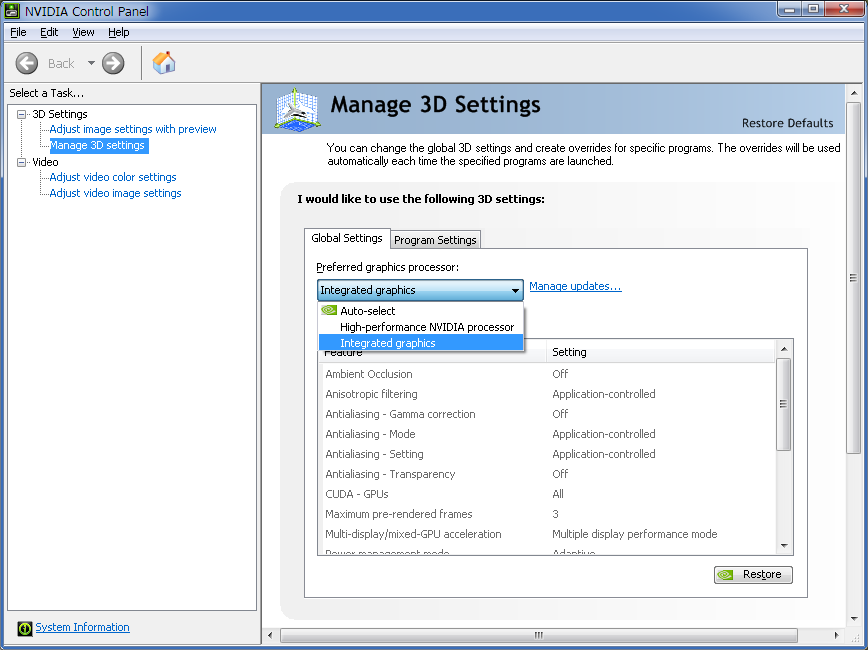
\includegraphics[width=7in]{nvidia_control_panel.png}
}
\caption{Nvidia Control Panel.}
\label{fig:imp}
\end{center}
\end{figure}

\subsection{My project does not show up on Eclipse's run (launch) button}
\label{p:missing_project}

\begin{enumerate}
\item Choose ``Organize Favorites'' from the bottom of the Run menu 
\item Press the "Add" button on the upper left of the resulting "Organize Run Favorites" window. 
\item Select all of the items in the ``Add Run Favorites'' window.
\end{enumerate}

\end{document}